%%%%%%%%%%%%%%%%%%%%%%%%%%%%%%%%%%%%%%%%%
% Beamer Presentation
% LaTeX Template
% Version 1.0 (10/11/12)
%
% This template has been downloaded from:
% http://www.LaTeXTemplates.com
%
% License:
% CC BY-NC-SA 3.0 (http://creativecommons.org/licenses/by-nc-sa/3.0/)
%
%%%%%%%%%%%%%%%%%%%%%%%%%%%%%%%%%%%%%%%%%

%----------------------------------------------------------------------------------------
% PACKAGES AND THEMES
%----------------------------------------------------------------------------------------

\documentclass[10pt,xcolor={dvipsnames}]{beamer}
%\setbeamersize{text margin left=1em,text margin right=1em}
\usepackage{mathtools}
\usepackage{amsmath}
\usepackage{bm}
\usepackage{hyperref}

\usepackage{graphicx} % Allows including images
\graphicspath{{/Users/rebecca/Documents/Rivet_Analyses/MC_VBFDM/PlotCombinationTool/Figures/}{/Users/rebecca/Documents/Presentations/Talks/}{/Users/rebecca/Documents/Rivet_Analyses/MC_VBFDM/PlotCombinationTool/Figures/StatPlots/}{/Users/rebecca/Documents/Rivet_Analyses/MC_VBFDM/PlotCombinationTool/Figures/2DHists/}{/Users/rebecca/Documents/JER/MinimiseMatrixJER/Difference_PowhegPythia/}{/Users/rebecca/Documents/Presentations/Reports/}}
\usepackage{booktabs} % Allows the use of \toprule, \midrule and \bottomrule in tables

\usepackage{etoolbox}
\usepackage{cancel}

\usepackage{subcaption}
\captionsetup{compatibility=false}

\usepackage{multirow}

\usepackage{appendixnumberbeamer}

%\newlength\origleftmargini
%\setlength\origleftmargini\leftmargini
%\setbeamertemplate{itemize/enumerate body begin}{\setlength{\leftmargini}{2pt}}%

%\let\oldexampleblock\exampleblock
%\let\oldendexampleblock\endexampleblock
%\def\exampleblock{\begingroup \setbeamertemplate{itemize/enumerate body begin}{\setlength{\leftmargini}{\origleftmargini}} \oldexampleblock}
%\def\endexampleblock{\oldendexampleblock \endgroup}%

%\let\oldalertblock\alertblock
%\let\oldendalertblock\endalertblock
%\def\alertblock{\begingroup \setbeamertemplate{itemize/enumerate body begin}{\setlength{\leftmargini}{\origleftmargini}} \oldalertblock}
%\def\endalertblock{\oldendalertblock \endgroup}

\mode<presentation> {

% The Beamer class comes with a number of default slide themes
% which change the colors and layouts of slides. Below this is a list
% of all the themes, uncomment each in turn to see what they look like.

%\usetheme{default}
%\usetheme{AnnArbor}
%\usetheme{Antibes}
%\usetheme{Bergen}
%\usetheme{Berkeley}
%\usetheme{Berlin}
\usetheme{Boadilla}
%\usetheme{CambridgeUS}
%\usetheme{Copenhagen}
%\usetheme{Darmstadt}
%\usetheme{Dresden}
%\usetheme{Frankfurt}
%\usetheme{Goettingen}
%\usetheme{Hannover}
%\usetheme{Ilmenau}
%\usetheme{JuanLesPins}
%\usetheme{Luebeck}
%\usetheme{Madrid}
%\usetheme{Malmoe}
%\usetheme{Marburg}
%\usetheme{Montpellier}
%\usetheme{PaloAlto}
%\usetheme{Pittsburgh}
%\usetheme{Rochester}
%\usetheme{Seahorse}
%\usetheme{Singapore}
%\usetheme{Szeged}
%\usetheme{Warsaw}

% As well as themes, the Beamer class has a number of color themes
% for any slide theme. Uncomment each of these in turn to see how it
% changes the colors of your current slide theme.

%\usecolortheme{albatross}
%\usecolortheme{beaver}
%\usecolortheme{beetle}
%\usecolortheme{crane}
%\usecolortheme{dolphin}
%\usecolortheme{dove}
%\usecolortheme{fly}
%\usecolortheme{lily}
%\usecolortheme{RoyalBlue}
%\usecolortheme{rose}
%\usecolortheme{seagull}
%\usecolortheme{seahorse}
%\usecolortheme{whale}
%\usecolortheme{wolverine}

%%Changing the theme colours
%\setbeamercolor*{structure}{bg=Plum!20,fg=Plum}
%\setbeamercolor*{palette primary}{use=structure,fg=white,bg=structure.fg}
%\setbeamercolor*{palette secondary}{use=structure,fg=white,bg=structure.fg!75}
%\setbeamercolor*{palette tertiary}{use=structure,fg=white,bg=structure.fg!50!black}
%\setbeamercolor*{palette quaternary}{fg=white,bg=black}
%\setbeamercolor{section in toc}{fg=black,bg=white}
%%\setbeamercolor{alerted text}{use=structure,fg=structure.fg!50!black!80!black}
%\setbeamercolor{titlelike}{parent=palette primary,fg=structure.fg!50!black}
%\setbeamercolor{frametitle}{bg=gray!30!white,fg=Plum}
%\setbeamercolor*{titlelike}{parent=palette primary}

%Changing the theme colours
\setbeamercolor*{structure}{bg=RoyalPurple,fg=RoyalPurple}
\setbeamercolor*{palette primary}{use=structure,fg=white,bg=structure.fg}
\setbeamercolor*{palette secondary}{use=structure,fg=white,bg=structure.fg}
\setbeamercolor*{palette tertiary}{use=structure,fg=white,bg=structure.fg}
\setbeamercolor*{palette quaternary}{fg=white,bg=black}
\setbeamercolor{section in toc}{fg=black,bg=white}
%\setbeamercolor{alerted text}{use=structure,fg=structure.fg!50!black!80!black}
\setbeamercolor{titlelike}{parent=palette primary,fg=structure.fg!50!black}
%\setbeamercolor{frametitle}{use=structure,fg=white,bg=structure.fg}
\setbeamercolor*{titlelike}{parent=palette primary}

%\setbeamercolor{block}{bg=yellow!10,fg=black}
%\setbeamercolor{block title}{bg=yellow!50,fg=black}
%\AtBeginEnvironment{block}{\setbeamercolor{itemize item}{fg=yellow}}

\newenvironment<>{examplefirst}[1]{%
  \setbeamercolor{block title}{bg=yellow!50,fg=black}%
  \begin{block}#2{#1}}{\end{block}}
\AtBeginEnvironment{examplefirst}{\setbeamercolor{itemize item}{fg=yellow}}

%\setbeamertemplate{footline} % To remove the footer line in all slides uncomment this line
%\setbeamertemplate{footline}[page number] % To replace the footer line in all slides with a simple slide count uncomment this line

%\setbeamertemplate{navigation symbols}{} % To remove the navigation symbols from the bottom of all slides uncomment this line


\setbeamertemplate{blocks}[rounded][shadow=false]
\setbeamertemplate{itemize items}[circle]
\setbeamertemplate{itemize subitems}[circle]

\renewcommand{\thefootnote}{\alph{footnote}}

}

%----------------------------------------------------------------------------------------
% TITLE PAGE
%----------------------------------------------------------------------------------------



\title[Project update]{Project update: Vector Boson Fusion to Dark Matter at the LHC and Jet Energy Resolution Determination} % The short title appears at the bottom of every slide, the full title is only on the title page

\author{\underline{Rebecca Pickles}, Darren Price} % Your name
%\institute[UoM] % Your institution as it will appear on the bottom of every slide, may be shorthand to save space
%{
%University of Manchester\\ % Your institution for the title page
%\medskip
%\textit{r.pickles@cern.ch} % Your email address
%}
% logo of my university
\titlegraphic{
\includegraphics[width=3cm]{UniOfManchesterLogo}}
\date{\today} % Date, can be changed to a custom date

\begin{document}

\begin{frame}
\titlepage % Print the title page as the first slide
\end{frame}

\iffalse
\begin{frame}
\frametitle{Overview} % Table of contents slide, comment this block out to remove it
\tableofcontents % Throughout your presentation, if you choose to use \section{} and \subsection{} commands, these will automatically be printed on this slide as an overview of your presentation
\end{frame}
\fi
%----------------------------------------------------------------------------------------
% PRESENTATION SLIDES
%----------------------------------------------------------------------------------------

%------------------------------------------------
\section{Introduction} % Sections can be created in order to organize your presentation into discrete blocks, all sections and subsections are automatically printed in the table of contents as an overview of the talk

%------------------------------------------------
\iffalse
\fi

\begin{frame}
\frametitle{Introduction}
\begin{block}{Jet Energy Resolution Determination}
\begin{itemize}
\item Investigating via the dijet balance method (using dijet events).
\item Important as jets are used as a tag for a large number of processes, including how $\cancel{E_{T}}$ is calculated.
\end{itemize}
\end{block}
\begin{exampleblock}{Vector Boson Fusion to Dark Matter at the LHC}
\begin{itemize}
\item Evaluating the sensitivity of the ATLAS Detector to observe Dark Matter through Vector Boson Fusion.
\item If Dark Matter preferentially couples to longitudinally polarised vector bosons, this will be the only way to detect it at the LHC.
\end{itemize}
\end{exampleblock}
\end{frame}

%-------------------------------------------------------------------------------

\section{JER}

%-------------------------------------------------------------------------------

\begin{frame}
\frametitle{JER: Dijet Balance Method}
\begin{itemize}
\item Uses the scalar balance between the momenta of the two leading jets and uses the presence of extra jets in data to calculate the sensitivity of the balance.
\item Two leading jets are expected to have equal transverse momentum, so any imbalance in p$_{T}$ must be due to the calorimeter. The Asymmetry describes this balance: \newline \newline
$
\mathcal{A} = \frac{p_{T}^{\mathrm{probe}} - p_{T}^{\mathrm{ref}}}{p_{T}^{\mathrm{avg}}} 
$
\item The width of this asymmetry distribution: \newline \newline
$
\sigma(\mathcal{A}^{\mathrm{probe}}) = \frac{\sqrt{\sigma^{2}(p_{T}^{\mathrm{ref}})+\sigma^{2}(p_{T}^{\mathrm{probe}})}}{p_{T}^{\mathrm{avg}}} 
$ 
\newline \newline
can be used to calculate the width of the p$_{T}$ of the probe jet: \newline \newline
$
\frac{\sigma(p_{T}^{\mathrm{probe}})}{(p_{T}^{\mathrm{probe}})} = \sqrt{\sigma^{2}(\mathcal{A}_{(i,i)}) - \frac{1}{2}\sigma^{2}(\mathcal{A}_{(i,j)})}
$
\end{itemize}
\end{frame}

\begin{frame}
\frametitle{JER: Determination of the JER}
\begin{itemize}
\item The jet energy resolution of the detector is found in data by subtracting the truth (particle-level) asymmetry from the reconstructed (measured) asymmetry. 
\item The truth asymmetry is found from event samples generated through a Monte Carlo. \newline \newline
$
\sigma({p_{T}}^{\mathrm{reco}}_{\mathrm{data}})=\sigma({p_{T}}^{\mathrm{det}}_{\mathrm{data}})\ast\sigma({p_{T}}^{\mathrm{physics}}_{\mathrm{data}})
$\newline \newline
$
\sigma({p_{T}}^{\mathrm{reco}}_{\mathrm{MC}})=\sigma({p_{T}}^{\mathrm{det}}_{\mathrm{MC}})\ast\sigma({p_{T}}^{\mathrm{physics}}_{\mathrm{MC}})
$\newline \newline
\item As $\sigma({p_{T}}^{\mathrm{physics}}_{\mathrm{data}})=\sigma({p_{T}}^{\mathrm{physics}}_{\mathrm{MC}})$ and $\sigma({p_{T}}^{\mathrm{reco}}_{\mathrm{data}})$ is known, $\sigma({p_{T}}^{\mathrm{det}}_{\mathrm{data}})$ can be found from: \newline \newline
$
\sigma({p_{T}}^{\mathrm{reco}}_{\mathrm{data}})=\sigma({p_{T}}^{\mathrm{det}}_{\mathrm{data}})\ast\sigma({p_{T}}^{\mathrm{physics}}_{\mathrm{MC}})
$
\end{itemize}
\end{frame}

\begin{frame}
\frametitle{JER: JER as a function of probe jet $\eta$}
Fractional jet p$_{T}$ resolutions obtained using the dijet balance method, shown as a function of $\eta_{\mathrm{det}}$ for data and MC.
\begin{columns}
\begin{column}{.5\textwidth}
\includegraphics[width=.8\linewidth]{55pTavg70_Difference.pdf} \newline
\includegraphics[width=.8\linewidth]{85pTavg115_Difference.pdf}
\end{column}
\begin{column}{.5\textwidth}
\includegraphics[width=.8\linewidth]{175pTavg220_Difference.pdf} \newline
\includegraphics[width=.8\linewidth]{400pTavg525_Difference.pdf}
\end{column}
\end{columns}
\end{frame}

\begin{frame}
\frametitle{JER: Further Progression}
\begin{itemize}
\item Assess a systematic on the subtraction from the spread of resolutions obtained from various MC samples.
\item Compare the MC detector resolution to those obtained from the subtraction and the data detector resolution.
\item Repeat the study with the bisector method:
\begin{itemize}
\item Separates out the part of the p$_{T}$ imbalance that is due to physics effects. 
\item Relies on different assumptions and so different sources of systematic uncertainty to the dijet balance method - Good validation. 
\end{itemize}
\end{itemize}
\end{frame}

%--------------------------------------------------------------------------------

\section{VBFDM}

%--------------------------------------------------------------------------------

\begin{frame}
\frametitle{VBFDM: Vector Boson Fusion}
Vector boson fusion (VBF) occurs when quarks from each proton in the collision produce W or Z bosons that interact. \newline
\begin{columns}
\begin{column}{.5\linewidth}
\center \includegraphics[width=0.9\textwidth]{VBF.pdf}
\end{column}
\begin{column}{.5\linewidth}
\begin{itemize}
\item Two hadronic jets are the main signature of VBF. 
\item VBF allows a broad coverage of mechanisms using an EFT.
\item VBF to DM is investigated using the ratio: \newline \newline
$
Ratio = \frac{\sigma((Z\rightarrow\cancel{E_{T}})jj)}{\sigma((Z\rightarrow l+ l-)jj)}
$
\newline \newline
Where $\cancel{E_{T}}$ could be neutrinos or possibly dark matter.
\item Signature for VBF DM is 2 jets and missing energy.
\end{itemize}
\end{column}
\end{columns}
\end{frame}

\begin{frame}
\frametitle{VBFDM: Background Events}
There are a number of different types of background for VBF DM events: Electroweak (EWK) initiated (Z $\rightarrow\nu\bar{\nu}$)jj; Quantum Chromo-dynamic (QCD) initiated (Z $\rightarrow\nu\bar{\nu}$)jj; QCD Multijet; and (W $\rightarrow \textrm{l} \nu$). 
\begin{columns}
\begin{column}{.4\linewidth}
\center{EWK} \newline
  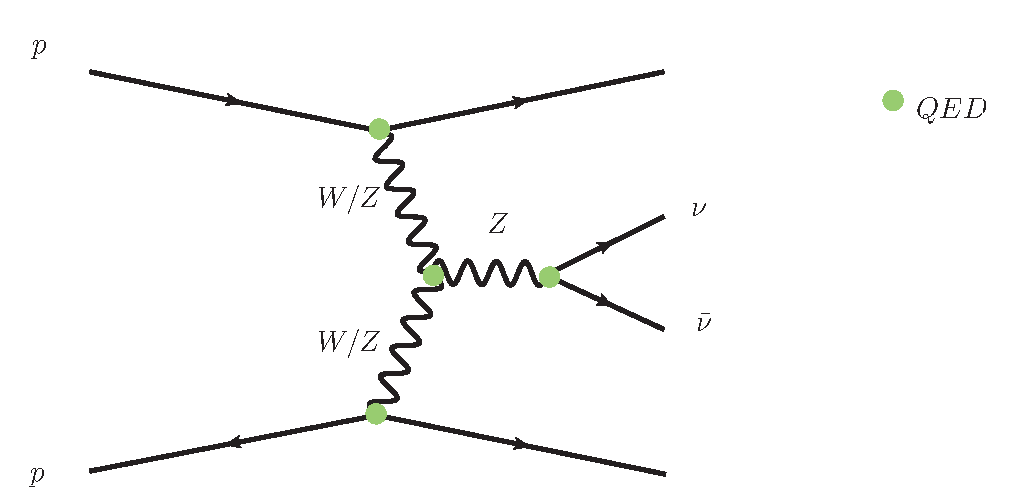
\includegraphics[width=.8\linewidth]{EWK_ppzjj_zvv}
  \newline
\end{column}
\begin{column}{.6\linewidth}
\center{QCD} \newline
  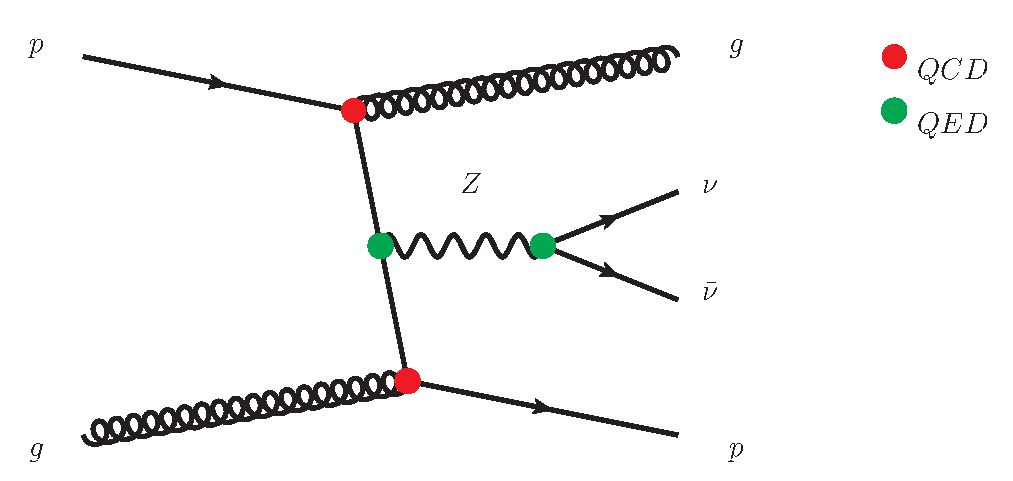
\includegraphics[width=.8\linewidth]{QCD_ppzjj_zvv}
  \newline
\end{column}
\end{columns}
\begin{itemize}
\item EWK: Neutrinos appear as missing transverse energy - could be DM.
\item QCD: Dominates the Zjj production and so needs to be known well.
\begin{itemize}
\item There are features to the QCD production of jets that allows it to be separated from the EWK. 
\end{itemize}
\end{itemize}
\end{frame}

\begin{frame}
\frametitle{VBFDM: QCD Multijet background}
This background is less well understood than other missing energy backgrounds as the missing energy is not down to 'real' physics, like neutrinos, where it can be estimated accurately from theory. If a jet is miss-measured in a unreliable part of the detector, or the resolution is not well measured, the other jets will be reconstructed incorrectly when trying to conserve momentum.
\begin{columns}
\begin{column}{0.5\linewidth}
\center
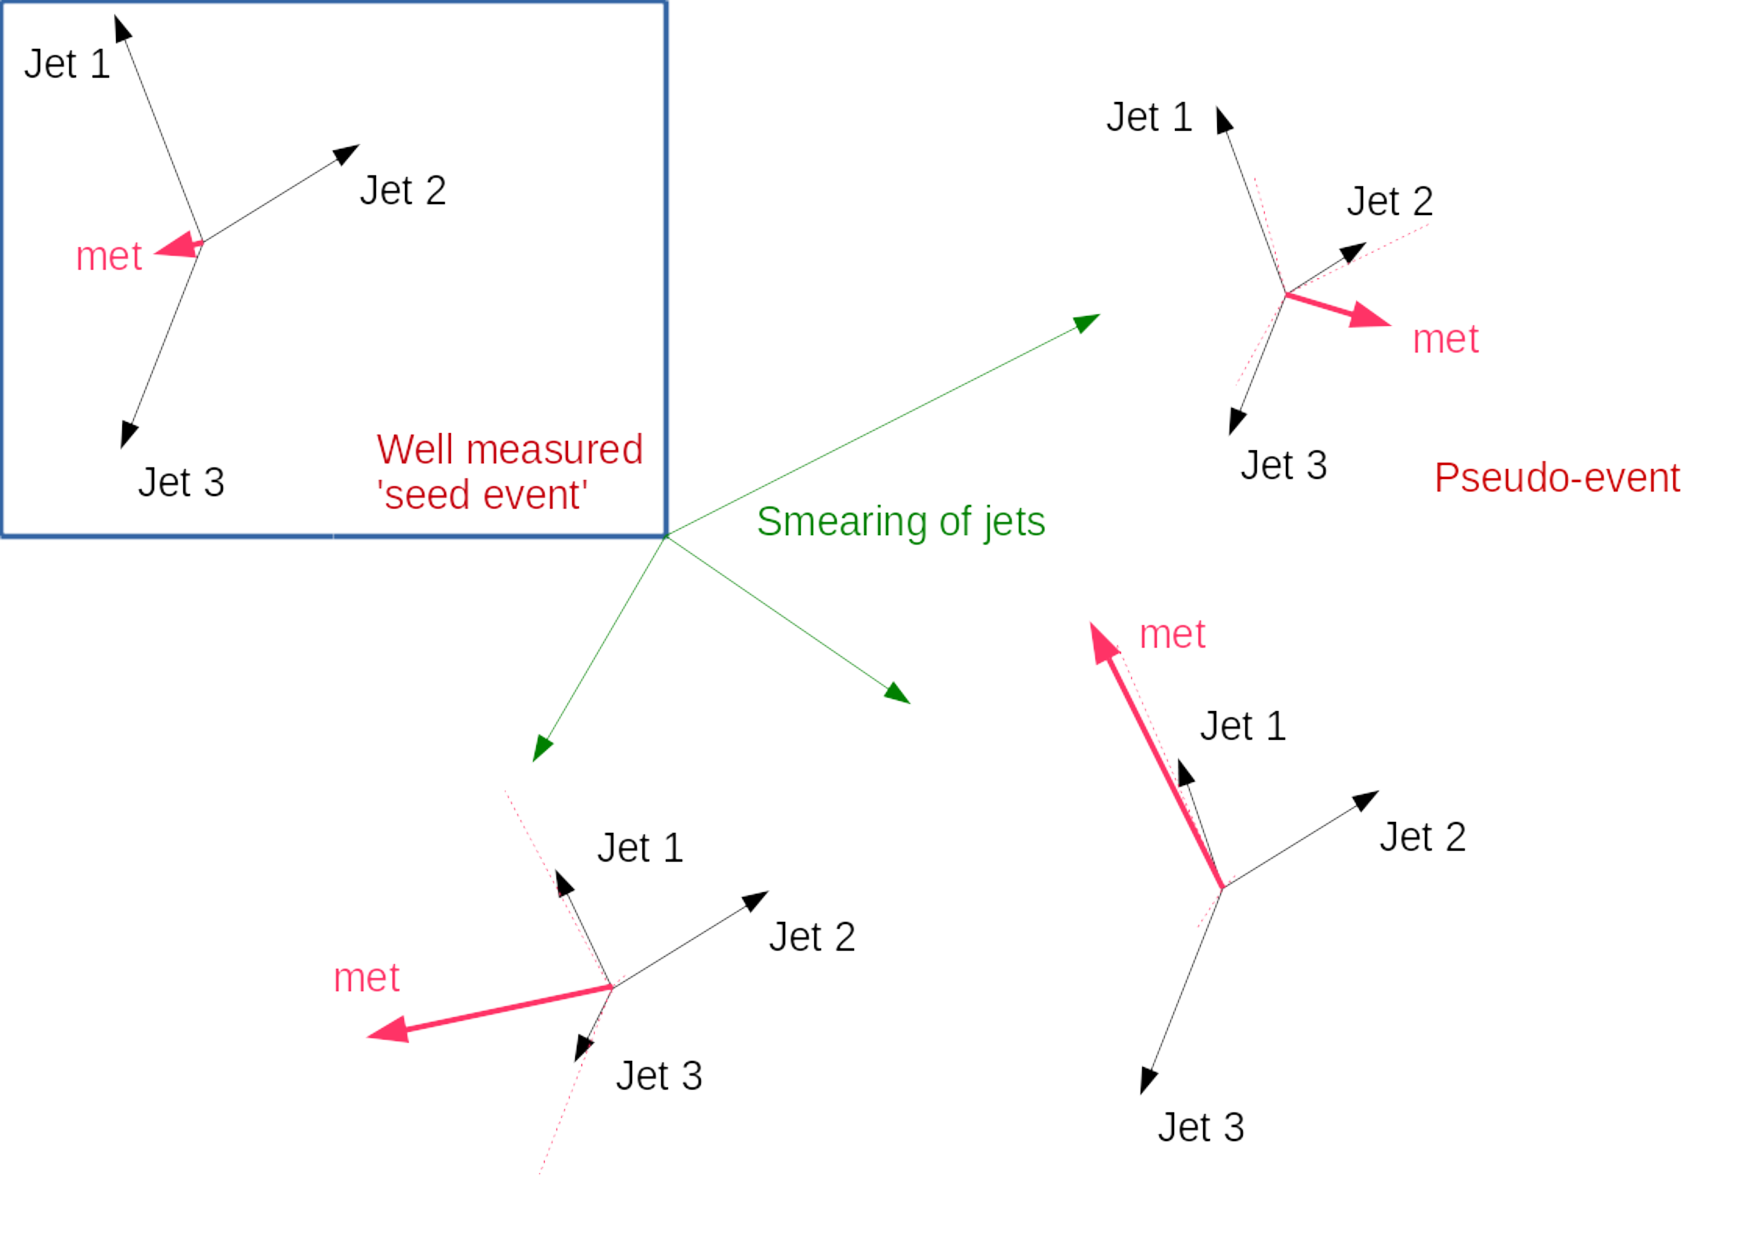
\includegraphics[width=6cm]{jetsmearing.pdf}
\end{column}
\begin{column}{0.5\linewidth}
\begin{itemize}
\item The idea behind jet smearing is create 'pseudo-data' which mimics events where the missing energy in an event mostly arises from the mis-measurement of jets.
\item This jet smearing uses the jet energy resolution work from the qualification task.
\end{itemize}
\end{column}
\end{columns}
\end{frame}

\begin{frame}
\frametitle{VBFDM: Jet energy resolution smearing method}
This is a data-driven method to find the mis-measured jet background of $\cancel{E_{T}}$ searches.
\begin{itemize}
\item Generate a large sample of jet seed events from MC, where jets are 'well-measured'. This is achieved by ensuring the reconstructed jet p$_{T}$ is as close as possible to the truth jet p$_{T}$. (Have access to MC and data inputs in the format necessary for this multijet smearing method from JER work.)
\item Use the resolution from JER dijet balance studies for p$_{T}^{avg}$ and $\eta$ bins.
\item Smear MC jet event 4-vectors according to a Gaussian with this resolution a large number of times to produce pseudo-data events.
\item Pass these pseudo-data events through the analysis cuts to produce the distributions. 
\end{itemize}
\end{frame}

\begin{frame}
\frametitle{VBFDM: MadGraph simulation using models}
\begin{itemize}
\item These processes are the ones being investigated in this analysis.
\item The black blobs represent the Effective Field Theories which are able to model the physics of heavy mediating particles between the standard model and DM fields. They give an approximation to an underlying theory, including the degrees of freedom appropriate to describe physical phenomena at a specific energy scale, but not specifying substructure and degrees of freedom at higher energies.
\end{itemize}
\begin{columns}
\begin{column}{.32\textwidth}
\center{EFT.}
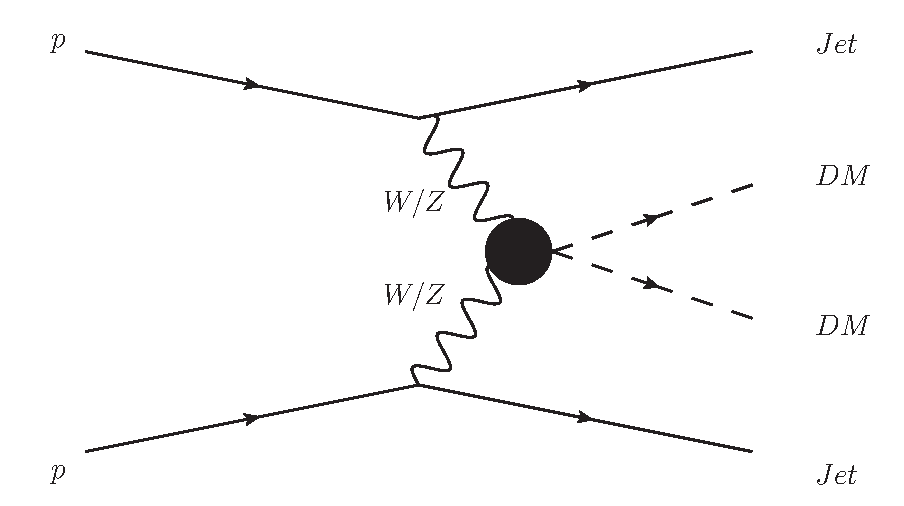
\includegraphics[width=1.\textwidth]{ppdmdmjj_feynman-eps-converted-to.pdf}
\newline
\end{column}
\begin{column}{.35\textwidth}
  \center{EFT from Z boson.}
\includegraphics[width=1.\textwidth]{ppdmdmjj_feynman_z}
\newline
\end{column}
\begin{column}{.30\textwidth}
  \center{With Higgs boson.}
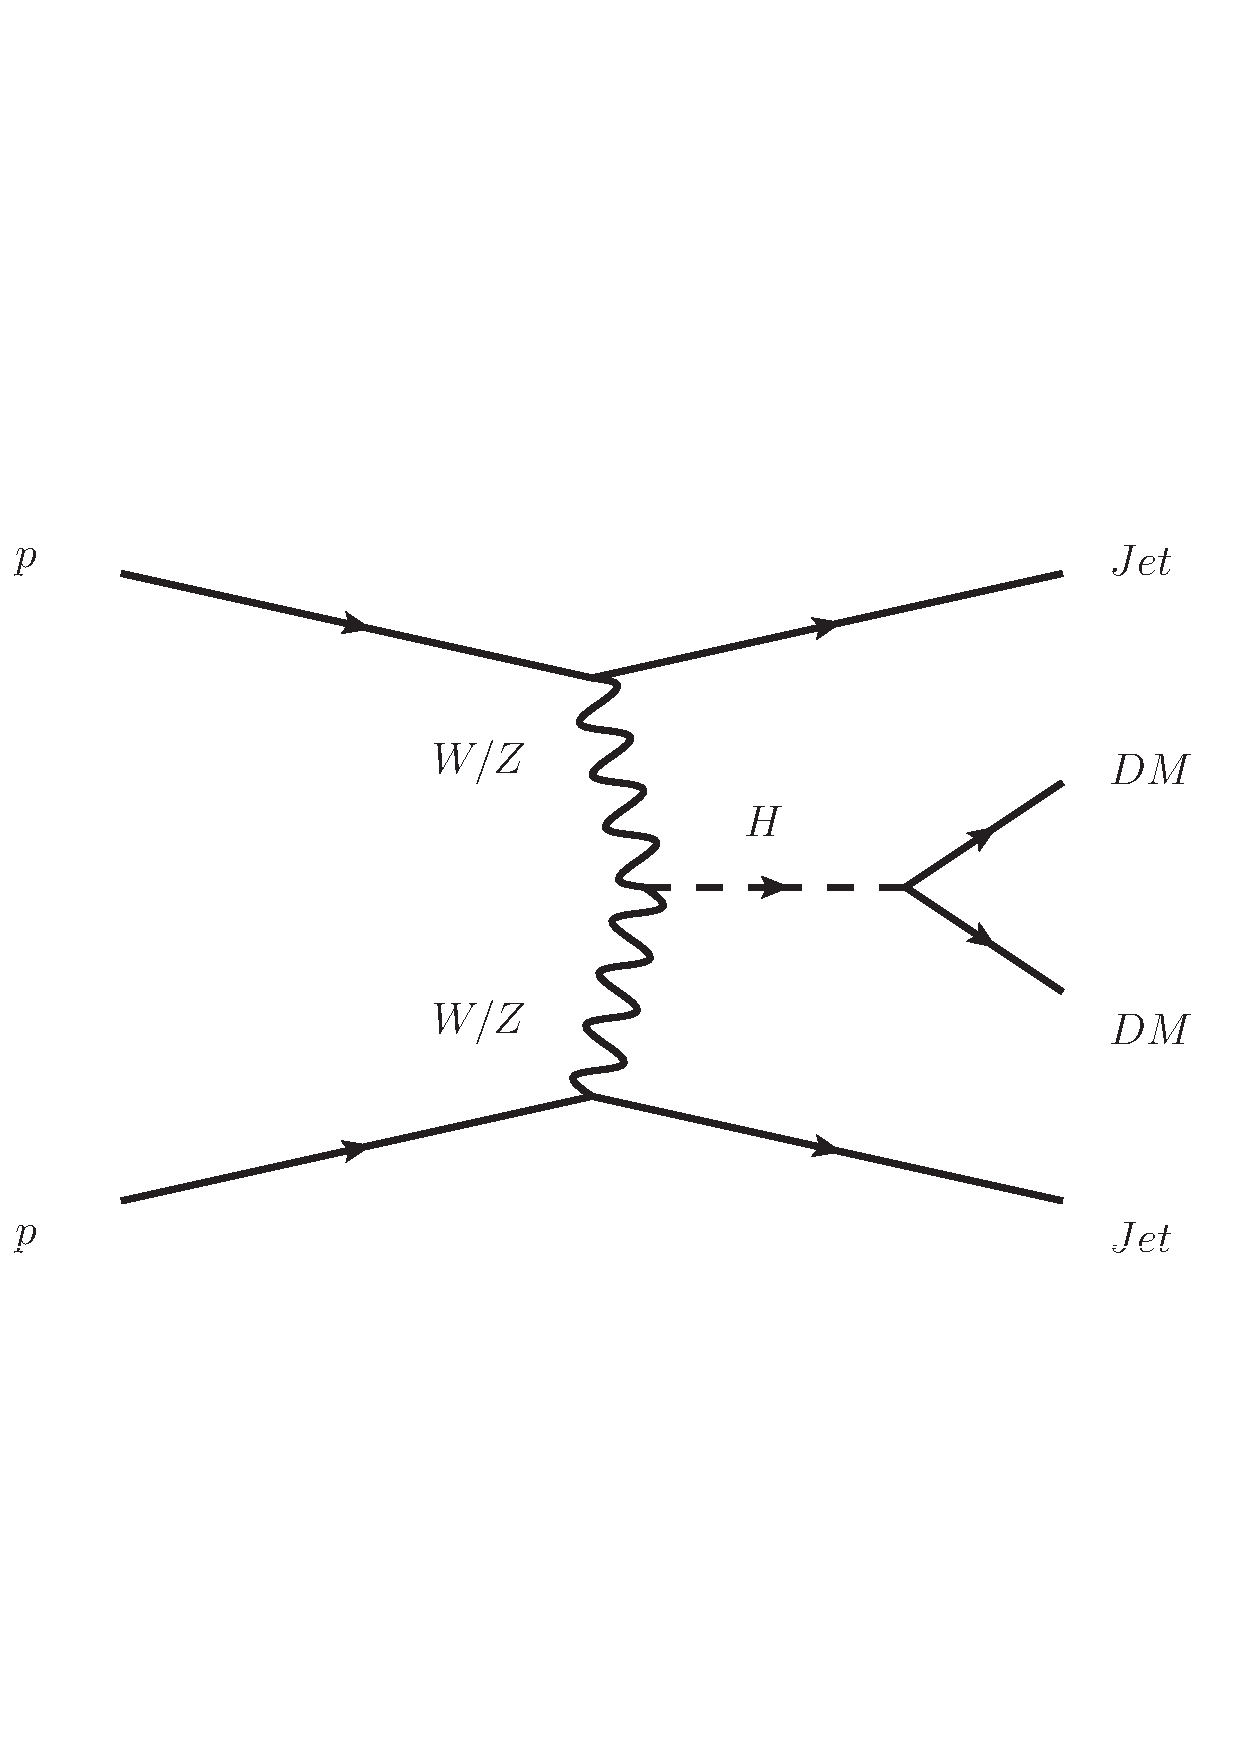
\includegraphics[width=1.\textwidth]{pphiggsdmdmjj}
\newline
\end{column}
\end{columns}
\begin{itemize}
\item MadGraph allows processes to be simulated within a framework defined by a Lagrangian.
\item Each of these Lagrangians gives a model that the process must work within.
\end{itemize}
\end{frame}

\begin{frame}
\frametitle{VBFDM: MadGraph simulation using models}
\begin{table}[H]
\begin{center}
\scriptsize
 \begin{tabular}{ c | c | c | c } 
 \hline \hline
 Name & Operator & Dimension & Minimum EFT Scale (GeV) \\ \hline \hline
 D5a & $\mathcal{L} = \frac{1}{\Lambda}\bar{\chi}\chi\bigg[\frac{Z_{\mu}Z^{\mu}}{2}+W_{\mu}^{+}W^{-\mu}\bigg]$ & 5 & 100 \\
 D5b & $\mathcal{L} = \frac{1}{\Lambda}\bar{\chi}\gamma^{5}\chi\bigg[\frac{Z_{\mu}Z^{\mu}}{2}+W_{\mu}^{+}W^{-\mu}\bigg]$ & 5 & 100 \\
 D5c & $\mathcal{L} = \frac{g}{2\cos{\theta_{W}}\Lambda}\bar{\chi}\sigma^{\mu\nu}\chi\bigg[\delta_{\mu}Z_{\nu}-\delta_{\nu}Z_{\mu}\bigg]$ & 5 & 3300 \\
 D5d & $\mathcal{L} = \frac{g}{2\cos{\theta_{W}}\Lambda}\bar{\chi}\sigma^{\mu\nu}\chi\epsilon^{\mu\nu\sigma\rho}\bigg[\delta_{\rho}Z_{\sigma}-\delta_{\sigma}Z_{\rho}\bigg]$ & 5 & 6600 \\
 D6a & $\mathcal{L} = \frac{g}{2\cos{\theta_{W}}\Lambda^{2}}\bar{\chi}\gamma^{\mu}\delta^{\nu}\chi\bigg[\delta_{\mu}Z_{\nu}-\delta_{\nu}Z_{\mu}\bigg]$ & 6 & 230 \\
 D6b & $\mathcal{L} = \frac{g}{2\cos{\theta_{W}}\Lambda^{2}}\bar{\chi}\gamma_{\mu}\delta_{\nu}\chi\epsilon^{\mu\nu\sigma\rho}\bigg[\delta_{\rho}Z_{\sigma}-\delta_{\sigma}Z_{\rho}\bigg]$ & 6 & 330 \\
 D7a & $\mathcal{L} = \frac{1}{\Lambda^{3}}\bar{\chi}\chi W^{i,\mu\nu}W_{\mu\nu}^{i}$ & 7 & 100 \\
 D7b & $\mathcal{L} = \frac{1}{\Lambda^{3}}\bar{\chi}\gamma^{5}\chi W^{i,\mu\nu}W_{\mu\nu}^{i}$ & 7 & 100 \\
 D7c & $\mathcal{L} = \frac{1}{\Lambda^{3}}\bar{\chi}\chi\epsilon^{\mu\nu\sigma\rho} W^{i,\mu\nu}W_{\rho\sigma}^{i}$ & 7 & 100 \\
 D7d & $\mathcal{L} = \frac{1}{\Lambda^{3}}\bar{\chi}\gamma^{5}\chi\epsilon^{\mu\nu\sigma\rho} W^{i,\mu\nu}W_{\rho\sigma}^{i}$ & 7 & 100 \\ \hline \hline
\end{tabular}
\end{center}
\end{table}
\begin{itemize}
\item \small{The rate of a process is proportional to $\Lambda^{-2(D-4)}$.}
\item \small{The different dimensions have the EFT scale constraints result in some dimensions with vastly reduced rates.}
\center{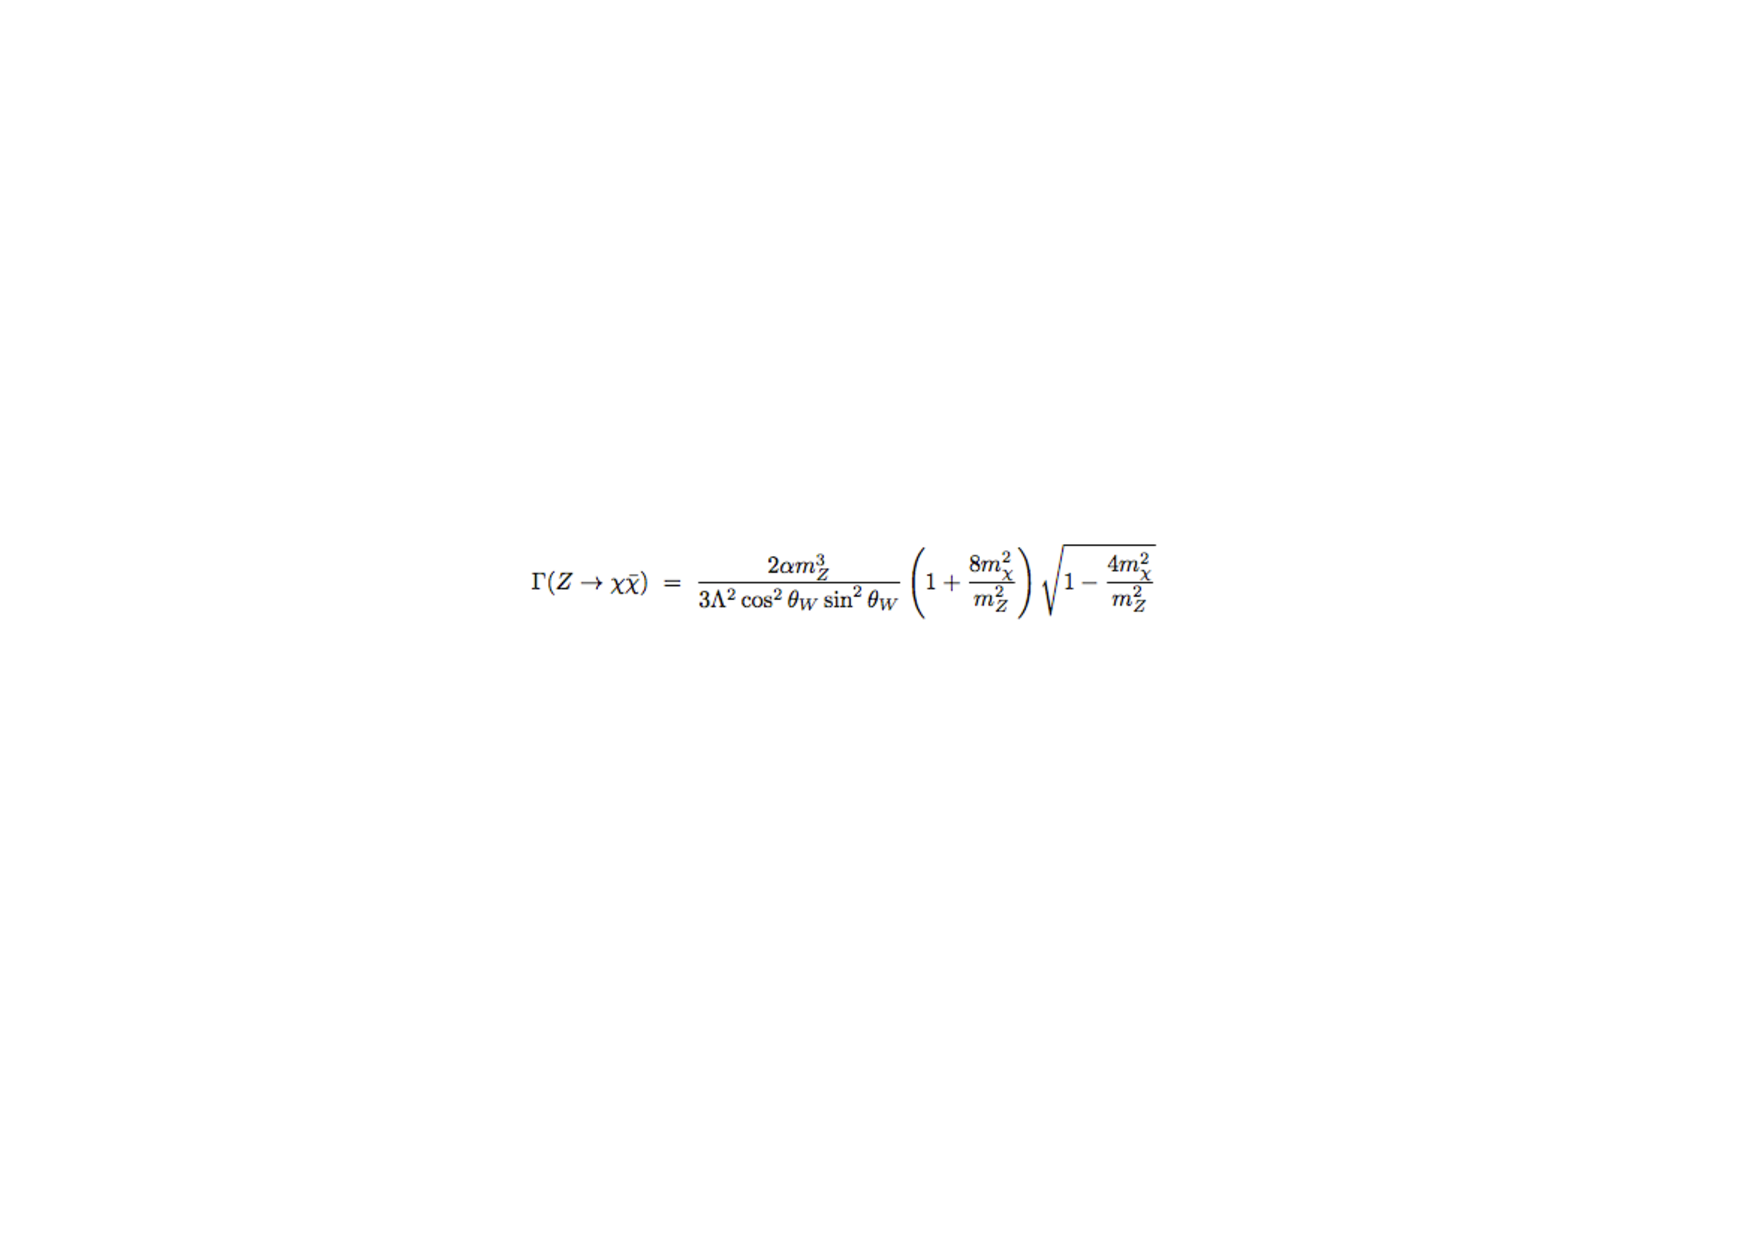
\includegraphics[width=0.5\linewidth]{D5a_Rate_Equation}}
\end{itemize}
\end{frame}


\begin{frame}
\frametitle{VBFDM: Rivet Analysis}
Rivet is specialised analysis software that includes the infrastructure to add user-made analyses. 
\begin{itemize}
\item Specialised rivet procedure processed the events produced in MadGraph.
\item It establishes cross-section distributions for a variety of phase-spaces, masses and observables.
\end{itemize}
\begin{table}[h!]
\begin{center}
\scriptsize
\begin{tabular}{ c | c  c  c  c  c  c} 
\hline \hline
Phase Space & Jet 1 p$_{T}$ & Jet 2 p$_{T}$ & $\mid\eta\mid$ & mjj & N$_{\mathrm{jets}}$ & $\cancel{\it{E}}_{T}$ \\
\hline \hline
VBFZ Baseline & \textgreater55 & \textgreater45 & \textless4.4 & n/a & \textgreater2 & n/a \\ 
VBFZ High-mass & \textgreater55 & \textgreater45 & \textless4.4 & \textgreater1000 & \textgreater2 & n/a\\ 
VBFZ Search & \textgreater55 & \textgreater45 & \textless4.4 & \textgreater250 & \textgreater2 & n/a \\ 
VBF Dark Matter & \textgreater55 & \textgreater45 & \textless4.4 & \textgreater250 & \textgreater2 & \textgreater150 \\ 
VBF DM High Jet p$_{T}$ & \textgreater100 & \textgreater45 & \textless4.4 & \textgreater250 & \textgreater2 & \textgreater150 \\
Monojet & \textgreater100 & n/a & \textless4.4 & n/a & \textgreater1 & \textgreater150 \\
Monojet High Jet p$_{T}$ & \textgreater100 & n/a & \textless4.4 & n/a & \textgreater1 & \textgreater250 \\
VBF DM or Monojet & \multicolumn{6}{| c }{ VBF DM or Monojet phase space cuts} \\
VBF DM or Monojet High Jet p$_{T}$ & \multicolumn{6}{| c }{ VBF DM or Monojet High Jet p$_{T}$ phase space cuts} \\
\hline \hline
\end{tabular}
\end{center}
\end{table}
\begin{itemize}
\item The VBF DM and Monojet phase-spaces are of most interest to this investigation.
\end{itemize}
\end{frame}

\begin{frame}
\frametitle{VBFDM: Model Kinematics and Rates}
\center{Normalised rate plot : DM Mass = 100GeV : Mjj : $\Lambda_{Min}$ = 100GeV} \newline
\begin{columns}
\begin{column}{.5\textwidth}
\includegraphics[width=6cm]{Mass100/Normalised/Mass100_Mjj_PS_VBFDM.pdf}
\end{column}
\begin{column}{.5\textwidth}
\begin{itemize}
\item Block colour shows EWK and QCD SM(Z$\rightarrow\nu\nu$)jj.
\item Effective operators with high EFT scale constraint have a very low rate.
\item The operators with the lowest EFT scale constraint have a higher rate than the background at high dijet mass.
\end{itemize}
\end{column}
\end{columns}
\end{frame}

\begin{frame}
\frametitle{VBFDM: Model Kinematics and Rates}
\center{Normalised rate plots : DM Mass = 100GeV : $\Lambda_{Min}$ = 100GeV} \newline
\begin{columns}
\begin{column}{.3\textwidth}
\includegraphics[width=4cm]{Mass100/Normalised/Mass100_Mjj_PS_VBFDM.pdf}
\end{column}
\begin{column}{.3\textwidth}
\includegraphics[width=4cm]{Mass100/Normalised/Mass100_Etmiss_PS_VBFDM.pdf}
\end{column}
\begin{column}{.3\textwidth}
\includegraphics[width=4cm]{Mass100/Normalised/Mass100_DeltaPhi_PS_VBFDM.pdf}
\end{column}
\end{columns}
\end{frame}

\begin{frame}
\frametitle{VBFDM: Ratio with Data and Observable Phase Space}
\center{Observable phase space and ratio plots : D5a : Mjj : $\Lambda_{Min}$ = 100GeV : 20\% statistical uncertainty}
\center
\includegraphics[width=10cm]{/D5a/Absolute/0.2/Stats_D5a_Mjj_02_PS_VBFDM.pdf}
\begin{itemize}
\item Observable phase space plot gives p-value from a $\chi^{2}$-test comparing the DM model to the SM background ratio of $\frac{\sigma((Z\rightarrow\nu\nu)jj)}{\sigma((Z\rightarrow\mu^{+}\mu^{-})jj)}$, for a range of DM masses and EFT scales.
\item Ratio plot shows $\frac{\sigma((Z\rightarrow\nu\nu)jj)+\sigma((Z\rightarrow DM DM)jj)}{\sigma((Z\rightarrow\mu^{+}\mu^{-})jj)}_{(EWK+QCD)}$
\end{itemize}
\end{frame}

\begin{frame}
\frametitle{VBFDM: Ratio with Data and Observable Phase Space}
\center{Observable phase space and ratio plots : D5a : Mjj : $\Lambda_{Min}$ = 100GeV : 2\% statistical uncertainty}
\center
\includegraphics[width=10cm]{/D5a/Absolute/0.02/Stats_D5a_Mjj_002_PS_VBFDM.pdf}
\begin{itemize}
\item Improved statistical uncertainty increases the range of the phase-space that can be excluded.
\end{itemize}
\end{frame}

\begin{frame}
\frametitle{VBFDM: Plans for 2D Observable phase space plots}
If two observables will give more sensitivity/exclude more observational phase space regions 2D plots could show what each observable excludes as well as what extra could be excluded when combining the sensitivities of both.
\begin{itemize}
\item Start with the dijet mass and jet $\Delta\Phi$ as they appear to give high p-values for different DM masses.
\item Look at which observables cover which EFT scales when the bug is fixed.
\end{itemize}
\end{frame}


\begin{frame}
\frametitle{Summary}
\begin{itemize}
\item JER:
\begin{itemize}
\item Made progress with the determination of the jet energy resolution
\item Aim to complete this work by summer for 2015 13TeV data.
\end{itemize}
\item VBF DM:
\begin{itemize}
\item Implemented a number of BSM models in MadGraph and used them to simulate the $Z\rightarrow\chi+\chi-$ process.
\item Produced a specialised Rivet procedure to analyse these simulated events and output cross-section distributions for a variety of phase-spaces, masses and observables.
\item Set up framework for statistical test of the DM models against all observables investigated.
\item Contributing to first general VBF DM search in ATLAS $\rightarrow$ Publish by summer for 13TeV.
\end{itemize}
\end{itemize}
\end{frame}




\end{document} 